\section{Asynchronous Programming}

\begin{description}
  \item[Task Continuations / CompletableFuture] can create chains of tasks that depend on each other. Wait at the end contradicts the idea, only necessary in special cases (keep main thread running for examples..).
  
  .NET: \texttt{task1
  .ContinueWith(task2)
  .ContinueWith(task3)
  .Wait();} 

  \texttt{Task.WhenAll(task1, task2).ContinueWith(task3);
  Task.WhenAny(task1, task2).ContinueWith(task3);}
  
  Java: \texttt{CompletableFuture
  .supplyAsync(() => firstOp)
  .thenApplyAsync(second)
  .thenAcceptAsync(third)};

  \texttt{CompletableFuture.allOf(future1, future2);
  CompletableFuture.any(future1, future2);}

  Use \texttt{exceptionally()} as Exception-Handling-Continuation
  \begin{figure}[H]
      \centering
      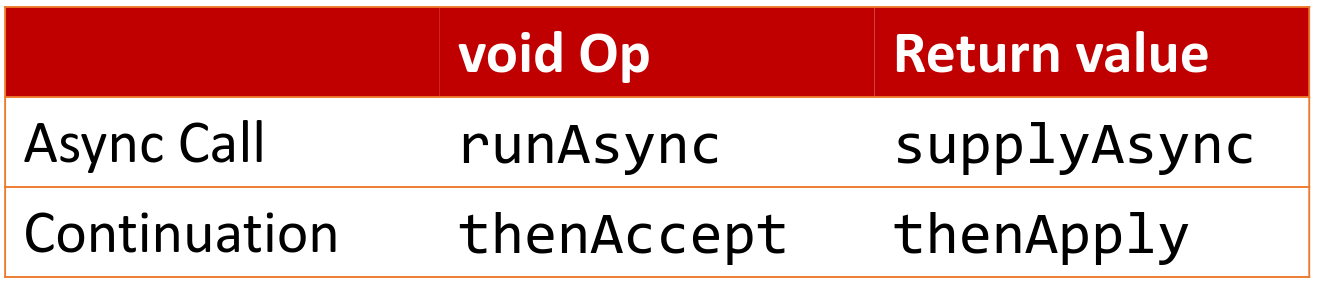
\includegraphics[width=10cm]{res/completable-future.png}
  \end{figure}
  
  \item[Caller-centric vs. Callee-centric] pull: caller requests result, push: callee (task) informs or continues once the result is available.
  
  \item[Exceptions] in Worker Tasks that are never awaited are ignored, in Java and .NET. No way of handling the exception is present. \texttt{TaskScheduler.UnobservedTaskException} could be used, but timing is GC-dependent.
  
  \item[Exceptionally] can be used in Java, similar to finally for try-catch.
\end{description}


\subsection{UI Programming}

Only a single UI Thread is allowed to do operations on UI components. The same thread should not execute long running operations, else the UI becomes unresponsive.

\begin{figure}[H]
  \centering
  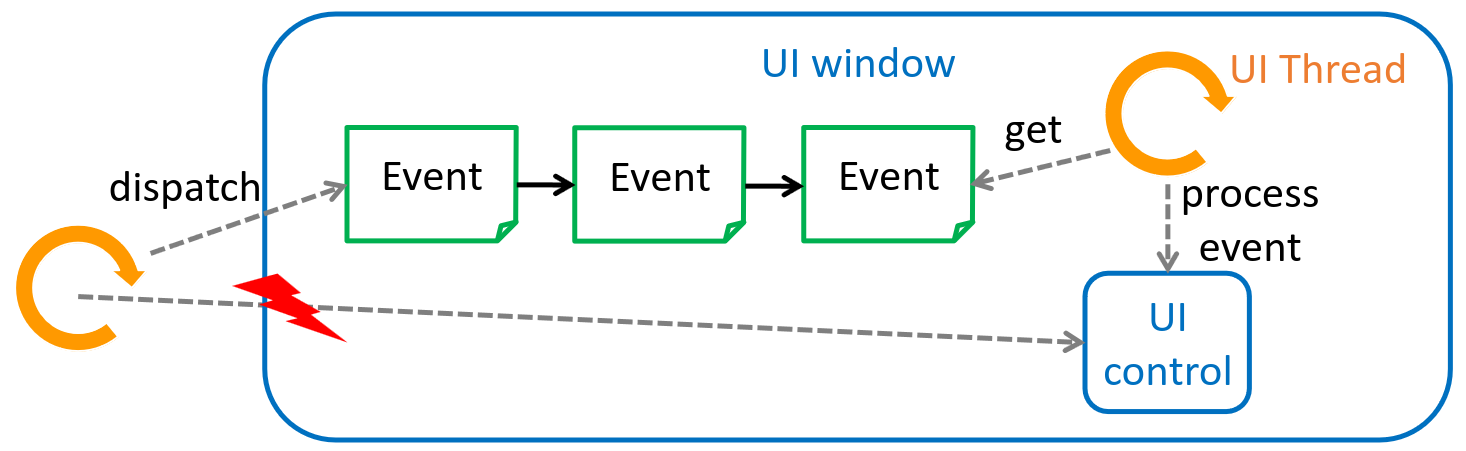
\includegraphics[width=12cm]{res/06-ui-thread-loop.png}
  \caption{UI Thread runs in a loop to process events}
\end{figure}

Logic in Java
\begin{lstlisting}
  button.addActionListener(event ->
    var url = textField.getText();
    CompletableFuture.runAsync(() -> {
      var text = download(url);
      SwingUtilities.invokeLater(() -> {
        textArea.setText(text);
      });
    });
  );
\end{lstlisting}

Logic in .NET
\begin{lstlisting}
  void buttonClick(...) {
    var url = textBox.Text;
    Task.Run(() => {
      var text = Download(url);
      Dispatcher.InvokeAsync(() -> {
        label.Content = text;
      });
    });
  }
\end{lstlisting}

Logic in .NET with async/await
\begin{lstlisting}
  var url = textBox.Text;
  var text = await DownloadAsync(url); // executes on worker thread
  label.Context = text;
\end{lstlisting}

Asynchronous methods are split up by the compiler. First part is run synchronously, code after the blocking call may be executed by another thread as a continuation.
If caller is a "normal" thread, execution is dispatched to another TPL worker thread. 
If caller is a UI thread, continuation is dispatched and processed as a UI event.

\subsection*{Async return value types}
\texttt{void}: fire and forget. 
\texttt{Task}: allows waiting for completion. 
\texttt{Task<T>}: allows waiting for a result of type T.
No support for \texttt{ref} or \texttt{out} parameters.

\vspace{3mm}
Async method must use await statement, else compiler will warn. Use tasks if necessary. Example:

\begin{lstlisting}
  public async Task<bool> IsPrimeAsync(long number) {
    return await Task.Run(() => {
      for (long i = 2; i * i <= number; i++) {
        if (number % i == 0) { return false; }
      }
      return true;
    });
  }
\end{lstlisting}